\documentclass{article}
\textheight 23.5cm \textwidth 15.8cm
%\leftskip -1cm
\topmargin -1.5cm \oddsidemargin 0.3cm \evensidemargin -0.3cm
%\documentclass[final]{siamltex}

\usepackage{verbatim}
\usepackage{fancyhdr}
\usepackage{amssymb,ctex}
\usepackage{mathrsfs}
\usepackage{latexsym,amsmath,amssymb,amsfonts,epsfig,graphicx,cite,psfrag}
\usepackage{eepic,color,colordvi,amscd}
\usepackage{enumerate}



\title{Numerical Analysis Homework2.1}
\author{Zhang Jiyao,PB20000204}

\begin{document}
	\maketitle
	
	\section{Introduction}
	对函数
	$$f(x)=\frac{1}{1+25x^2},x\in [-1,1]$$
	构造$Newton$插值多项式$p_L(x)$,插值节点取为:
	$$1.x_i=1-\frac{2}{N}i,i=0,1,...,N$$
	$$2.x_i=-cos(\frac{2i+1}{2N+2}\pi),i=0,1,...,N$$
	并计算如下误差
	$$max_i\{\left|f(y_i)-p(y_i)\right|,y_i=\frac{i}{50}-1,i=0,1,...,100\}$$
	并且对$N=5,10,20,40$比较以上两组节点的结果,并在一张图中画出$N=20$时$f(x)$数值计算结果.
	
	
	\section{Method}
	本次实验采用MATLAB进行编程.一共有两个文件,一个是函数文件,用于计算$Newton$插值多项式,另一个是用于计算以及输出结果的。
	考虑使用$Newton$插值法构造插值多项式.对不同的$N$,根据给出的数据点,构造插值多项式来逼近。然后对所有节点遍历,求出最大误差。
	
	\section{Results}
	
	\begin{figure}[p]
		\begin{center}
			
			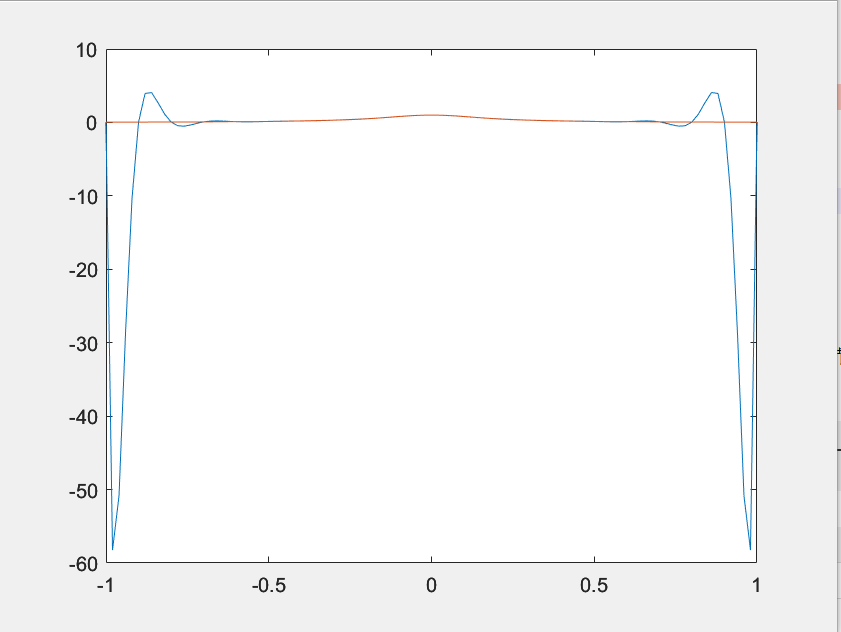
\includegraphics[width=10cm,height=10cm]{graph}
			
			\caption{当N=10时的图像} \label{figure.label}
		\end{center}
	\end{figure}
	
	\begin{figure}[p]
		\begin{center}
			
			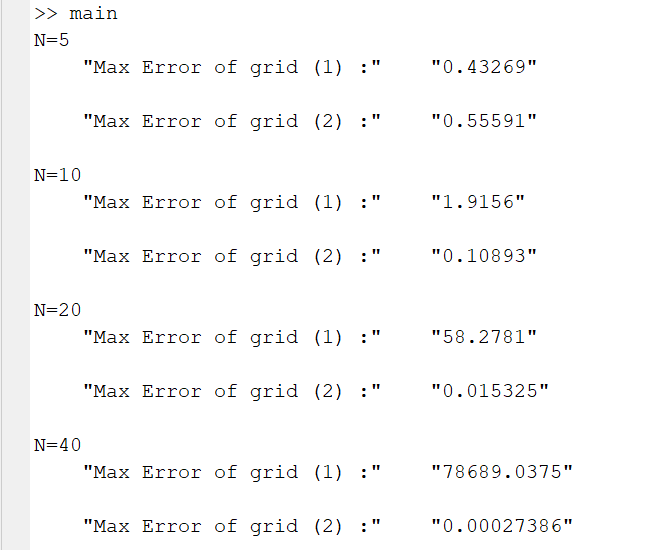
\includegraphics[width=10cm,height=10cm]{result}
			
			\caption{输出结果} \label{figure.label}
		\end{center}
	\end{figure}
	
	
	\section{Discussion}
	
	
	观察到第一组节点的拟合效果较差。当$N$越大时,误差反而越大.而第二组节点的拟合效果整体就较好.当$N$越大时,逼近效果更好,误差较小。大概是第一组节点取值比较均匀,不能有效反映出函数的所有信息,所以会在一个局部出现较大的误差.而第二组节点取值相对随机一点,更有效的反映出函数的全部信息。
	
	\section{Computer Code}
	\verbatiminput{Newton.m}
	\verbatiminput{main.m}
	
	
\end{document}